\documentclass[11pt]{article}
\usepackage{acl-hlt2011}
\usepackage{url}
\usepackage{latexsym}
\usepackage{epsfig}
\usepackage{latexsym}
\usepackage[usenames]{color}
\usepackage{times} 
\usepackage{verbatim}
\usepackage{multirow}
\usepackage{threeparttable}
\usepackage{booktabs}
\usepackage{subfig}
\usepackage{graphicx}
\usepackage[small,compact]{titlesec}
\usepackage{amsmath}
\usepackage{color}

\usepackage[]{algorithm2e}


% For figure placement
\def\topfraction{.9}
\def\textfraction{0.07}  %allow pages with minimal text and more figure space.
\def\floatpagefraction{.9}

% For reducing space between bib entries
\let\oldthebibliography=\thebibliography
  \let\endoldthebibliography=\endthebibliography
  \renewenvironment{thebibliography}[1]{%
    \begin{oldthebibliography}{#1}%
      \setlength{\parskip}{0ex}%
      \setlength{\itemsep}{0ex}%
  }%
  {%
    \end{oldthebibliography}%
  }

\begin{document}

\author{David Jurgens$^{1,2}$\\
  $^{1}$HRL Laboratories, LLC\\
  Malibu, California, USA\\
  {\tt jurgens@cs.ucla.edu}
  \And
  Keith Stevens$^{2}$ \\
  $^2$University of California, Los Angeles\\
  Los Angeles, California, USA\\
  {\tt kstevens@cs.ucla.edu}}

\title{Measuring the Impact of Sense Similarity on Word Sense Induction}

\date{}

\maketitle

\begin{abstract}
Word Sense Induction (WSI) is an unsupervised learning approach to discovering
the different senses of a word from its contextual uses.  
A core challenge to
WSI approaches is distinguishing between related and possibly similar senses of
a word.  Current WSI evaluation techniques have yet to analyze the specific
impact of similarity on accuracy.
Therefore, we present a new WSI evaluation that quantifies the relationship
between the relatedness of a word's senses and the ability of a WSI algorithm to
distinguish between them.  Furthermore, we perform an analysis on sense
confusions in SemEval-2 WSI task according to sense similarity.
% 
Both analyses for a representative selection of clustering-based WSI approaches
reveals that performance is most sensitive to the clustering algorithm and not
the lexical features used.

\end{abstract}
  
\section{Introduction}

Many words in a language have several distinct meanings.  For example, ``earth''
may refer to the planet Earth, dirt, or solid ground, depending on the context.
The goal of Word Sense Induction (WSI) is to automatically discover the
different senses by examining how a word is used.  This unsupervised discovery
process produces a sense inventory where the number of senses is corpus-driven
and where senses may reflect additional usages not present in a predefined sense
inventory, such as those for medicine or law \cite{dorow03discovering}.
Furthermore, these discovered senses can be used to automatically expand lexical
resources such as WordNet or FrameNet \cite{klapaftis10taxonomy}.

Discovering the multiple senses is frequently confounded by the relationships
between a word's senses.  While homonyms such as ``bass'' or ``bank'' have
unrelated senses, many polysemous words have interrelated senses, with
lexicographers often in disagreement for the number of fine-grained senses
\cite{palmer07making}.  For example, the most frequent four senses for ``law''
according to WordNet, shown in Table \ref{tab:law-senses}, are similar in
several aspects and could be ascribed interchangeably in some contexts.
%
The difficulty of automatically distinguishing two senses is proportional to
their similarity because of the increasing likelihood of the two senses sharing
similar contexts.


While the issue distinguishing between related senses is a recognized issue 
for Word Sense Disambiguation \cite{chugur02polysemy,mccarthy06relating}, which
uses supervised training to learn sense distinctions, measuring the impact of
sense relatedness on the harder problem of WSI remains unaddressed.
%
The recent SemEval WSI tasks \cite{agirre07semeval,manandhar09semeval} have
provided a standard framework for evaluating WSI systems, with a controlled
training corpus designed to limit sense ambiguity in the example contexts.
However, given the potential relatedness of a word's senses, we view it
necessary to consider how WSI methods perform relative to the degree of
contextual ambiguity.
%
Our goal is therefore to quantify the similarity at which a WSI approach is
unable to distinguish between two senses, which reflects the sense granularity
at which the approach operates.

\begin{table}
  \footnotesize
  \begin{tabular}{l p{70mm}}
    \toprule
    1 & the collection of rules imposed by authority \\
    2 & legal document setting forth rules governing a particular kind of activity \\
    3 & a rule or body of rules of conduct inherent in human nature and essential to or binding upon human society \\
    4 & a generalization that describes recurring facts or events in nature \\
    \bottomrule
  \end{tabular}
  \caption{Definitions for the top four senses of ``law'' according to WordNet}
  \label{tab:law-senses}
\end{table}

We propose two new evaluations.  The first, described in Section
\ref{sec:related-senses}, uses a similarity-based pseudo-word discrimination
task to measure the discrimination capability for related senses along a graded
scale of similarity.  As a second evaluation, in Section \ref{sec:semeval} we
perform an error analysis using the SemEval-2010 WSI task, examining sense
confusion relative to the sense similarities.  For both evaluations, we examine
twenty different WSI clustering-based models through combining five feature
types and four clustering algorithms.  These models were selected to be
representative of a wide class of existing algorithms as a way of influence
future algorithmic directions based on the current model's performance.

\section{Clustering Contexts to Discover Senses}
\label{sec:clustering}

Frequently, WSI is treated as an unsupervised clustering problem: The contexts
in which a word appears are clustered in order to discover its senses
\cite{navigli09word}.  
We selected four diverse clustering algorithms for evaluation based on three
criteria: (1) the ability to automatically determine the final number of
clusters given an upper bound or a set of parameters, (2) an efficient run time,
and (3) high quality results in either WSI or other fields related to text
analysis.  The first criteria is essential for WSI; the final number of senses
must be derived without supervision in order to reflect the true number of
senses present in the corpus.

\paragraph{K-Means}
K-Means builds clusters based on the similarity between two data points.
Clusters grow by assigning data points to the cluster with the most similar
centroid.  After every data point is assigned, each cluster's centroid is
recalculated to be the average of all the data points assigned to the cluster.
This process repeats until the centroids converge to a fixed point.  We choose
initial seeds at random and use the H2 criterion function
\cite{zhao02criterionfunctions}.  Although K-Means is efficient and widely used,
it requires the number of clusters to be specified a priori.  Therefore, we
follow the WSI model of \newcite{pedersen06automaticcluster} and use the Gap
Statistic \cite{tibshirani00estimating} to automatically determine the number of
clusters.

The Gap Statistic runs K-Means repeatedly with different values of $K$, ranging
from 1 to some sensible maximum.  The Gap Statistic first induces a data model
from the feature distributions of the initial dataset and then for each $K$,
creates a set of artificial datasets by sampling from the derived model.  $K$ is
increased until the ``gap'', i.e.  the distance between the objective function
of the original dataset and the average objective function of the artificial
datasets, is larger then the gap for the previous $K$ value.  We calculate the gap using
10 artificial data sets sampled from the model.

\paragraph{Spectral Clustering}
%
Spectral Clustering interprets a dataset's elements as vertices in graph with
edges based on their similarity \cite{ng01spectral}.  Clusters are found by
identifying the graph partition that produces the minimum conductance between
every partition.  This can be thought of as trying to find small islands that
are connected by as few bridges as possible.  We refer the reader to
\cite{von07tutorial} for further technical details. To our knowledge, only
\newcite{he10applying} have applied spectral clustering to WSI, which was
performed on a Chinese dataset.  However, the algorithm used by He et
al.\ requires the number of clusters to be specified.

We instead use a hybrid spectral clustering algorithm, first applied to
information retrieval \cite{cheng06divide}, that automatically selects the
number of clusters.  This algorithm recursively partitions a dataset in half by
finding the cut that produces the minimum conductance, which builds a tree of
partitions.  This split is done until either every data point is in its own
partition or a maximum number of partitions is found.  Partitions are then
dynamically merged, starting at leaf partitions, based on a clustering criteria.
We use the relaxed correlation criteria \cite{cheng06divide},
which tries to maximize both inter cluster similarity and intra cluster
dissimilarity.  The final cluttering generated is then the best tree-respecting
partition of the original data set.

\paragraph{Clustering By Committee}
Pantel and Lin \shortcite{pantel02discovering} found that K-Means clustering
folded all features found in a cluster into the centroid, many of which are not
useful for identifying the desired word sense.  To overcome this, they proposed
a novel clustering algorithm for WSI, Clustering by Committee (CBC), which
includes only the most distinguishing features for a cluster into the centroid.

For each context, an initial set of ``committees'' is formed by clustering the
most similar contexts to each context, with the resulting committees ranked to
prefer larger, highly similar clusters.  The final set of committees (sense
clusters) are selected by recursively identifying the highest ranking committees
that are dissimilar to each other and then repeating the process for any
contexts not similar to existing committees.  In essence, CBC aims to find the
clusters that are similar to the largest set of contexts, while keeping clusters
dissimilar from each other.  CBC's recursion ensures that contexts dissimilar to
the large committees are still grouped into their own smaller committees, which
enables the discovery of infrequent senses with distinct contexts.  We use a
hard sense assignment for each context, i.e., a context is labeled with only one
sense according to the most similar cluster.

\paragraph{Streaming K-Means}
As WSI moves into inducing senses from Web-scale amounts of data, existing
clustering algorithms that keep all contexts in memory become impractical.
Jurgens and Stevens \shortcite{jurgens10hermit} proposed an on-line hybrid
clustering solution using on-line K-Means and Hierarchical Agglomerative
Clustering, which automatically decided the number of clusters without retaining
all the contexts.  To the best of our knowledge, theirs is the only work using
an on-line approach.  We extend this work by applying a more theoretically sound
online K-Means algorithm, called Streaming K-Means \cite{braverman11streaming},
to WSI.  We use Streaming K-Means to conduct a direct algorithmic comparison
with K-Means in the hopes that online approaches can be made just as effective
as off-line approaches.

Streaming K-Means processes each data point only once, thus reducing the memory
overhead dramatically.  Instead of recording each data point, it immediately
assigns each data point to a cluster and maintains $K \cdotp C$ clusters.  $C$ varies
as the algorithm runs, initially being set to 0.  When assigning a data point,
it is only assigned to an existing cluster when their similar is above some
threshold, otherwise the data point becomes the centroid of a new cluster.  Once
$C$ reaches a threshold, based on an estimate of the number of data points, or
the overall K-Means clustering cost reaches some limit, the centroids are
treated as new data points and re-clustered, with the goal of merging some
centroids.  We follow \cite{jurgens10hermit} and cluster the final centroids
with Hierarchical Agglomerative Clustering, with the average link criteria as
suggested by \cite{pedersen97distinguishing}.

\section{Modeling Context}
\label{sec:context}

For each clustering algorithm, we consider five context models that represent
the types of lexical features used by the majority of WSI approaches.

\paragraph{Co-Occurrence} 
Contexts formed from word co-occurrence are the most common in WSI algorithms.
For each occurrence of a word, those words within a certain range are counted as
features. Prior work has used a variety of context sizes, e.g. words in the same
sentence \cite{bordag06word}, in nearby lexical positions
\cite{gauch93experiments}, or within a paragraph-sized context window 
\cite{pedersen10duluth}.

We consider two co-occurrence context models: a 5-word and a 25-word window.  We
note that in co-occurrence-based word space algorithms, smaller context sizes
have shown to better capture paradagmatic similarity, while larger sizes capture
semantic associativity \cite{peirsman08size,utsumi10exploring}.

\paragraph{Dependency-Relations}

Dependency parsing creates a syntax tree where words are directly linked
according to their relation.  These links refine co-occurrence based contexts by
utilizing syntactic indications of how words are related.  Dependency parsed
features have proven highly effective for word representations in many NLP
applications, e.g., \cite{pado07dependency,baroni10strudel}.  We follow
\newcite{pantel02discovering} and \newcite{dorow03discovering} using the
sentence as contexts and all words with a dependency path of length 3 or less,
with the last word and its relation as a feature.  We note that recently
\newcite{kern10kcdc} achieved good WSI performance with only a small,
manually-tuned subset of all relations as context.


\paragraph{Word Ordering}
Word ordering can provide a mild form of syntactic information
\cite{jones06high,sahlgren08permutations}.  While other syntactic features may
provide significantly more information, word ordering is efficient to compute
and provides an alternative source of syntactic information for knowledge-lean
systems or for languages where NLP tools are not readily available.  

Because we treat word ordering as a syntactic feature, we limit the context to
words occurring in the same sentence.  A feature is the combination of a
co-occurring word and its relative position, i.e. the same word in different
positions is treated as two separate features.

\paragraph{Parts of Speech}
Part of speech tagging can provide a preliminary coarse-grained sense
disambiguation of a word's contextual features, where a word may have as many
senses as it does parts of speech.   For example, consider an occurrence
of ``house'' in the context of ``address'' as a noun and verb: ``I went to his
house address,'' and ``I heard the legislator address the house.''
%
Labeling ``address'' with its part of speech provides for more semantic
information on its meaning, which further constrains the sense of ``house.''
%
Prior work \cite{pedersen97distinguishing} has suggested that this information
can improve performance, but to our knowledge, the impact of POS features has
not been evaluated in isolation.

Each context is formed from the containing sentence; a feature is a combination
of each word and its part of speech, e.g., ``board-NOUN'' is distinct from
``board-VERB.''

\section{WSI Performance on Related Senses}
\label{sec:related-senses}

\newsavebox{\tempbox}
\begin{figure*}
  \vspace{-4mm}
  \centering
  \subfloat[5-Word Co-Occurrence]{\label{fig:co5}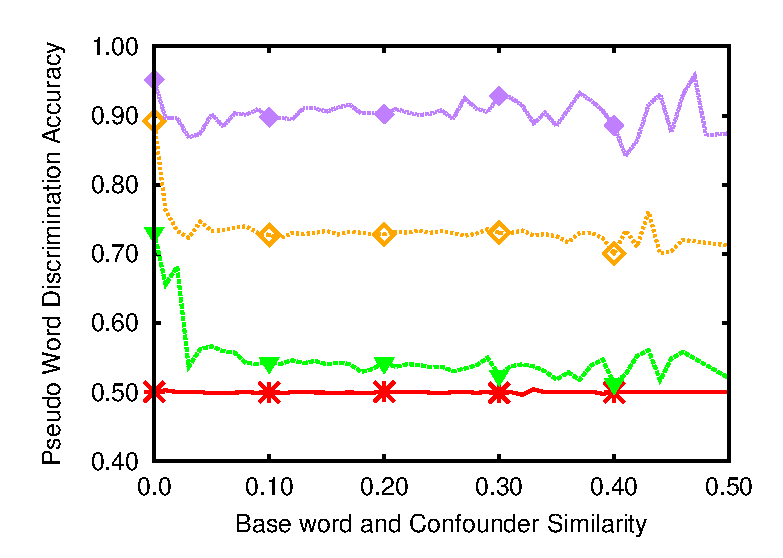
\includegraphics[width=0.33\textwidth]{figures/cooccurrence-5w-pwd-results.eps}}
  \subfloat[25-Word Co-Occurrence]{\label{fig:co20}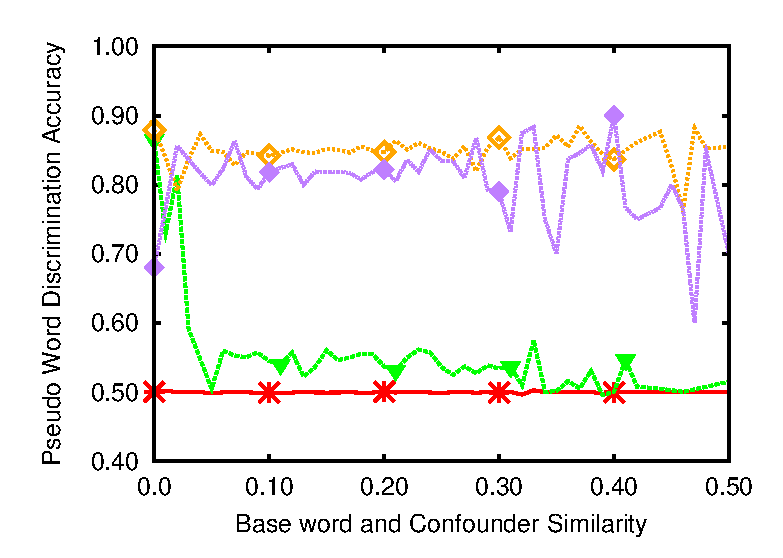
\includegraphics[width=0.33\textwidth]{figures/cooccurrence-20w-pwd-results.eps}} 
  \subfloat[Dependency Relations]{\label{fig:dp}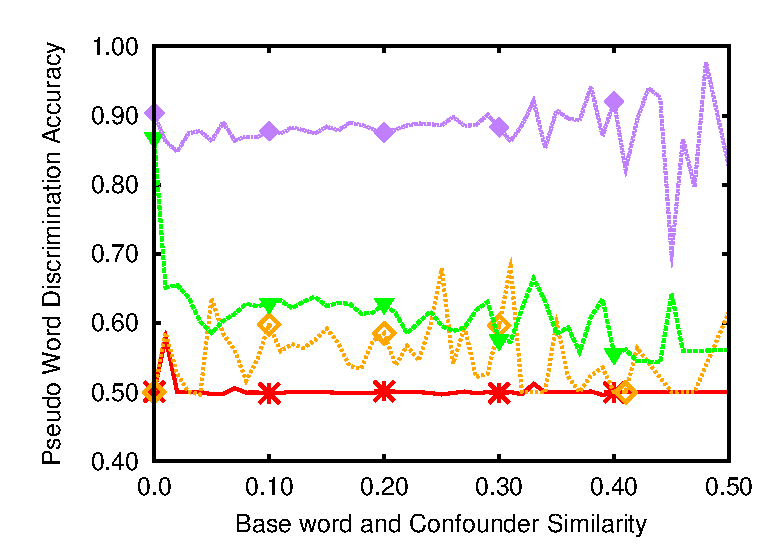
\includegraphics[width=0.33\textwidth]{figures/dv-pwd-results.eps}} \\
  \subfloat[Word Order]{\label{fig:order}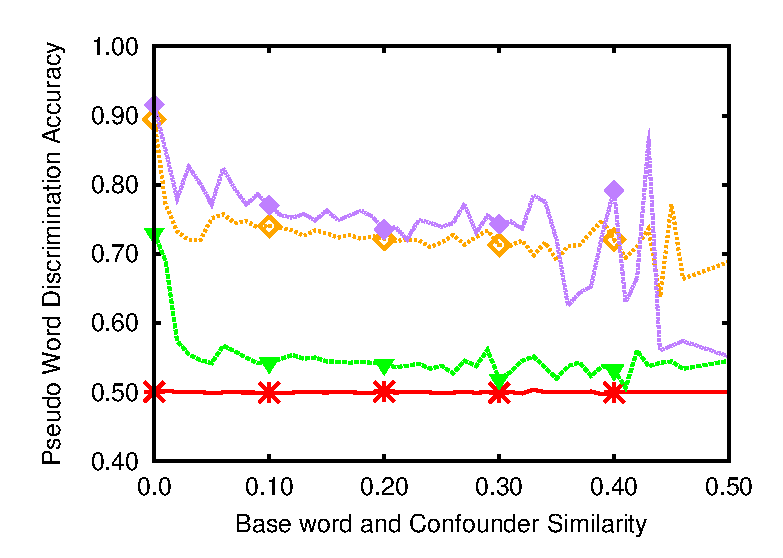
\includegraphics[width=0.33\textwidth]{figures/pos-order-results.eps}} 
  \subfloat[Parts of Speech]{\label{fig:pos}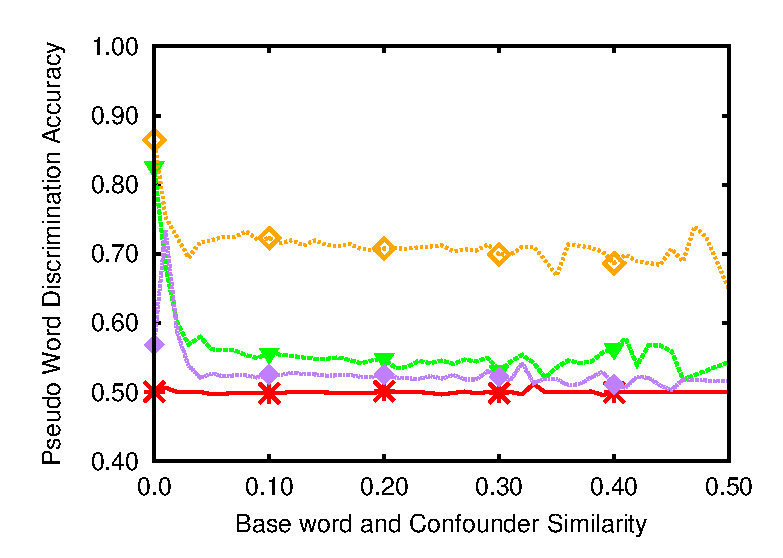
\includegraphics[width=0.33\textwidth]{figures/pos-pwd-results.eps}} 
  \subfloat[]{
    \label{fig:key}
    % BEWARE: HERE BE LOTS O' BLACK MAGIC...
    \vbox{% 
      \vfil
      \hspace{-161mm}
      \vspace{12mm}
      \includegraphics[width=0.008\textwidth]{figures/key-test.eps}
      \vfil}
  }%
  \caption{Pseudo-word discrimination performance }
  \label{fig:pwd-results}
\end{figure*}


The proposed methodology measures the ability of a WSI approach to distinguish
between related senses.  However, generating a large corpus with manually
labeled sense assignments and sense similarity judgements is prohibitively
expensive.  Therefore, we employ a pseudo-word discrimination task
where a base word and a second word, its \emph{confounder}, are replaced
throughout the corpus with a pseudo-word.  The objective is then to determine
which of the words was originally present given the context of an occurrence of
the pseudo-word.  Due to not requiring manual annotation, this type of task
was initially proposed as a substitute for word sense disambiguation
\cite{schutze92context,gale92work} and for selectional
preferences \cite{clark02class}.



\begin{table}[tb]
  \footnotesize
  \center
  \begin{tabular}{ll l ll}
    \toprule
    \multicolumn{2}{c}{\textbf{festival}} && \multicolumn{2}{c}{\textbf{laws}} \\
        \cmidrule{1-2} \cmidrule{4-5} 
    offices    & 0.13660 && interests   & 0.18289 \\
    play       & 0.13751 && politics    & 0.20440 \\
    convention & 0.20296 && governments & 0.29125 \\
    tournament & 0.29007 && regulations & 0.40761 \\
    concerts   & 0.48348 && legislation & 0.56112 \\
    \bottomrule
  \end{tabular}
  \caption{Example confounders for ``festival'' and ``laws'' and their similarities}
  \label{tab:example-confounders}
\end{table}

Following the suggestions of \newcite{chambers10improving} on designing
pseudo-words, pseudo-words were created from words with the same part of
speech and equal frequency in the training corpus.  We selected nouns occurring
more than 5,000 times in a 2009 Wikipedia snapshot and then drew 5,000 contexts
for each.  The snapshot was tagged with the Stanford Part of Speech Tagger
\cite{toutanova03feature} and parsed with the Malt Parser
\cite{nivre06maltparser}.

To evaluate the impact of sense similarity, pseudo-words were created from word
pairs with a broad range of lexical similarities.  We selected lexical
similarity as an approximation of sense similarity in order to model the
hypothesis that similar senses may appear in similar contexts.
Similarity scores were calculated using cosine similarity on contextual
distributions built from a sliding $\pm2$ word window over the Wikipedia corpus.
Table \ref{tab:example-confounders} highlights several example confounders and
their similarities with the base term.  In total, we generated 5000
term-confounder pairs from 98 base terms, with a mean of 51 confounders per
term.

All clustering parameters were chosen using the default values provided in the
original papers. K-means and Streaming K-Means were both set with a maximum of
15 clusters, with the final number of clusters being determined by the data
itself.


\subsection{Evaluation}

The pseudo-word's senses are induced from a training segment using each feature
and clustering combination.  
%
Given that both words making up the pseudo-word may be polysemous, more than two
senses may be induced.
%
Each sense cluster is labeled according to which of the original words was
present in the majority of its contexts. For testing, each instance of the
pseudo-word in a previously unseen context is assigned the label of the cluster
to which it is most similar.  We perform five-fold cross-validation, using 4,000
contexts for training and 1,000 contexts for testing.  Discrimination accuracy
is reported as the average of all five runs.  Since an equal number of contexts
are used for each term, the base line accuracy of a most frequent sense model is
50\% for each pseudo-word.

\subsection{Results and Discussion}

Figure \ref{fig:pwd-results} shows the discrimination accuracy relative to the
similarity of a base pair and confounder, for each feature and clustering
algorithm combination.  Similarity values were binned at the 0.01 level with a
mean of 39.0 scores per bin
(median=11).  Because most word pairs are not related, the
  distribution of similarity values is biased towards lower values.  
Therefore, we omit similarity ranges above 0.5, as too few confounders occurred
in that range to draw reliable conclusions.  The standard error (not shown) is
$< 1$ for all measurements.

The general trends suggests that the clustering algorithm impacts the sense
discriminatory ability far more than the lexical feature choice.  Furthermore,
sense similarity affects most clustering algorithms, with most systems seeing a
noticeable performance drop when pseudo-word similarity is increased just beyond
0.  Performance at high similarity becomes more variable for all algorithms and
features.

For each clustering algorithm, we see dramatically different trends.  
%
Streaming K-Means performs well with co-occurrence based features and it does
poorly when either contexts have too many features, as in the 25 Window
Co-Occurrence feature space, or the feature space overall is too sparse, as in
the Parts of Speech and Ordering feature spaces.

K-Means with the gap statistic converges to the most frequent sense baseline for
nearly every confounder pair.  We note that this behavior significantly differs
from that seen in \cite{pedersen06automaticcluster}, which clustered
second-order co-occurrence vectors rather than the first-order features that we
use.  Our analysis showed that the H2 criterion was responsible for this
behavior.  A subsequent analysis revealed that K-Means still converged to MFS
for the E1, E2, I1, and I2 criterion functions \cite{zhao02criterionfunctions}
as well as when the number of artificial datasets was increased up to 100.
However, additional tests using the same features on the SemEval-1 WSI task did
not converge to MFS.  Further investigation is needed to identify the cause of
convergence and what types of data are appropriate the Gap Statistic.

Clustering by Committee performs well on most models, but significantly worse on
dependency relation features.  A subsequent analysis showed that CBC
generates significantly more clusters than all other models.  For the POS, 5
word window, and 25 window Co-Occurrence feature spaces, CBC generated between
205 and 247 clusters on average, per word.  With the order feature space, CBC
generated 1087 clusters per word.  However, when paired with dependency relation
features, the number of clusters drops to only 78 per word.  

Spectral Clustering is most affected by sense similarity, performing
competitively for unrelated senses but dropping significantly when words become
even slightly similar.  This performance drop is seen across all features.
Performance is therefore low, with the exception of dependency relations.

Overall, these results suggest that sense relatedness is a important factor in
WSI performance and its impact should be considered in future WSI evaluations.
A potential next step is to vary the proportion of contexts from the confounder.
The current method intentionally uses a uniform distribution to avoid potential
bias; however, word sense distributions are rarely equal, and a varied
distribution would more closely model real world distributions.  Similarly, the
current method tested only two senses, whereas an n-way disambiguation between
multiple confounders should also provide further insight into a WSI approach's
discriminatory abilities.

\section{Sense Confusion in SemEval-2 Task 14}
\label{sec:semeval}

As a second experiment, we analyze incorrect sense assignments on SemEval-2 Task
14 \cite{manandhar10semeval} to measure whether sense-relatedness biases which
sense was incorrectly selected. For WSI systems, a similarity bias would
indicate that similar senses are more likely to be incorrectly identified as a
single sense.

We summarize Task 14 as follows.  Systems are provided with an unlabeled
training corpus consisting of 879,807 multi-sentence contexts for 100 polysemous
words, comprised of 50 nouns and 50 verbs.  Systems induce sense representations
for target words from the training corpus and then use those representations to
label the senses of the target words in unseen contexts from a test corpus.

The induced senses are then evaluated against the gold standard labels OntoNotes
\cite{hovy06ontonotes} senses labels for the test corpus.  For our evaluation,
we use both the two contrasting unsupervised measures, the paired FScore
\cite{artilse09role} and the V-Measure \cite{rosenberg07vmeasure}, and a
supervised measure.  For each metric, we use the evaluation framework provided by the organizers of
SemEval-2 Task 14.\footnote{\tiny\url{http://www.cs.york.ac.uk/semeval2010_WSI/}}

The V-Measure rates the homogeneity and completeness of a
clustering solution.  Solutions that have word clusters formed from one
gold-standard sense are homogeneous; completeness measures the degree to which a
gold-standard sense's instances are assigned to a single cluster.
%
The paired FScore measures two types of overlap of a solution and the gold
standard in cluster assignments for all in pair-wise combination of instances.
This score tends to penalize solutions with many small clusters and highly
heterogeneous clusters \cite{manandhar09semeval}.  

The supervised evaluation measures the recall when building a Word Sense
Disambiguation classifier from the induced senses.  The WSI system labels the
entire corpus, which is then divided into training and test portions.  The sense
labels in the training portion are used to construct a mapping from induced
senses to the gold standard OntoNotes labels.  This mapping is then evaluated
for the induced labels in the test.  We report the scores for the 80\% training
and 20\% testing scenario.

\begin{figure*}[t!f]
  \vspace{-5mm}
  \center

  \subfloat[Streaming K-means]{\label{fig:stkm+co}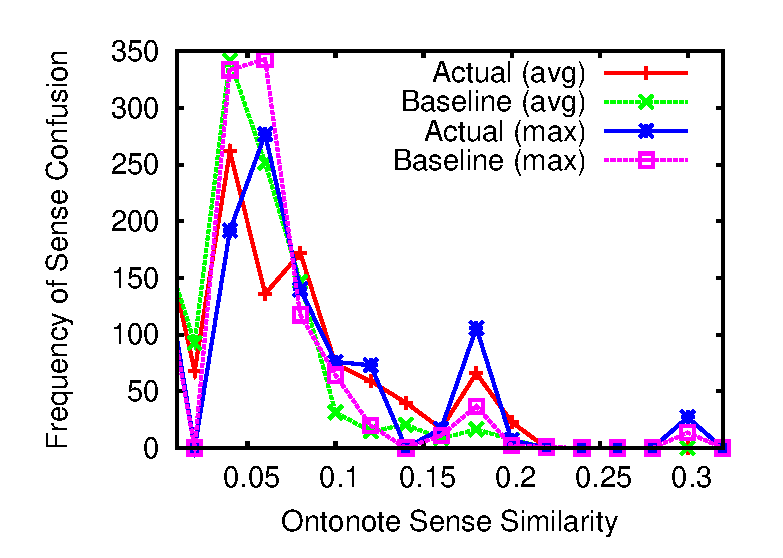
\includegraphics[width=.45\textwidth]{code/plots/semEval-2010-dv-wc-wordsi-stkm-test.key.eps}}
  \subfloat[CBC]{\label{fig:stkm+wo}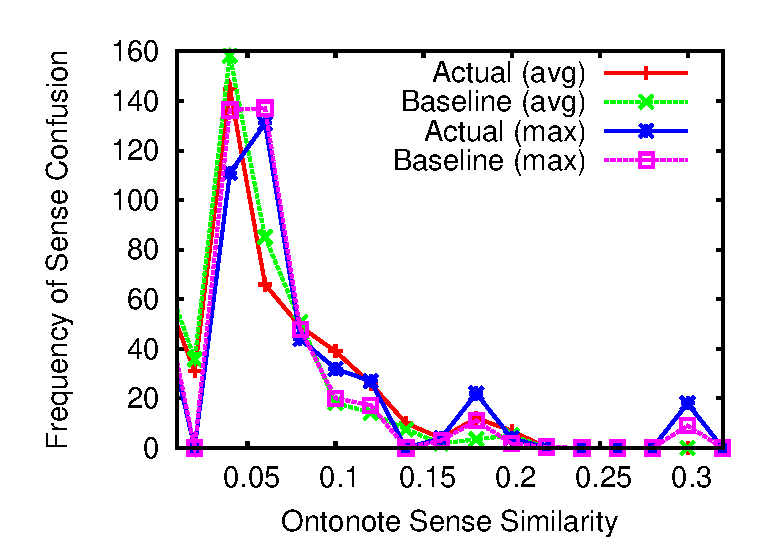
\includegraphics[width=.45\textwidth]{code/plots/semEval-2010-dv-wc-wordsi-cbc-test.key.eps}} \\
  \subfloat[Spectral Clustering]{\label{fig:sc+co}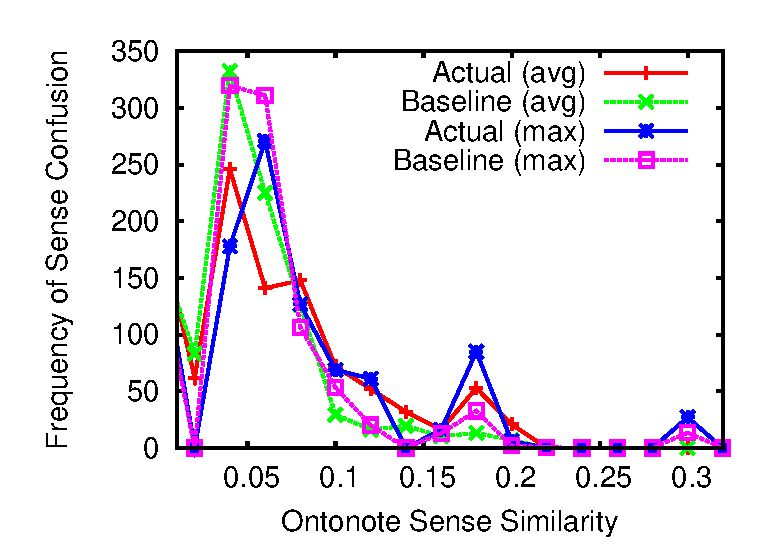
\includegraphics[width=.45\textwidth]{code/plots/semEval-2010-dv-wc-wordsi-sc06-test.key.eps}} 
  \subfloat[K-means]{\label{fig:km+co}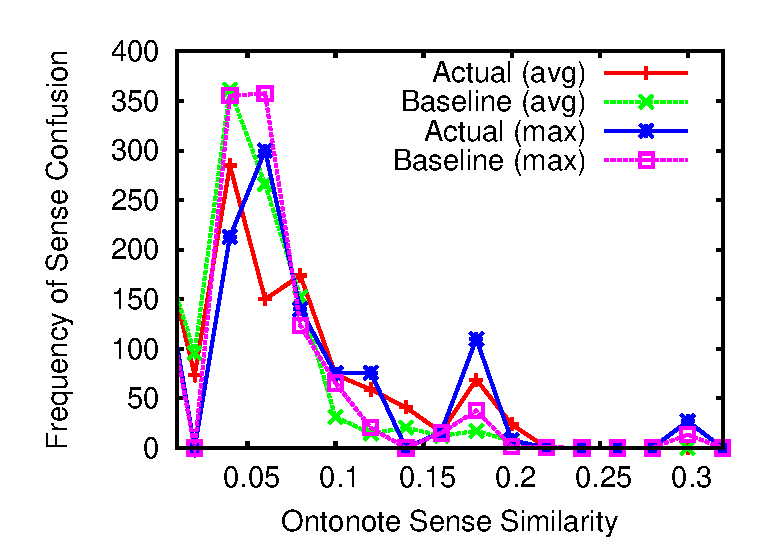
\includegraphics[width=.45\textwidth]{code/plots/semEval-2010-dv-wc-wordsi-gs-kmeans-test.key.eps}} \\

  \caption{The error frequency distributions for confusing the correct sense
    with another sense of the given similarity when using a 5-word co-occurrence
    window as context.  Dashed lines indicate the null models. }
  \label{fig:sense-confusion}
\end{figure*}


\begin{table*}[!ftb]
  \center
  \footnotesize
  \begin{tabular}{ c  c  c  c  c  c c l }
  \toprule
  \textbf{Context Feature} & \textbf{Clustering} &
  \textbf{V-Measure} & \textbf{F-Score} &
  \textbf{Recall} & \textbf{\# Clusters}  &
  \textbf{Purity} & \textbf{GoF p-Value} \\
  \midrule
    \multirow{4}{*}{5-Word Co-Occurrence}
& Streaming & 6.7 & 55.5 & 54.8 & 4.74 & 0.103& p $<$ 2.07e-37 \\
& Spectral & 10.8 & 39.2 & 54.3 & 8.41 & 0.194& p $<$ 1.11e-25 \\
& CBC & 23.9 & 8.2 & 39.5 & 39.7 & 0.665& p $<$ 0.916\\
& K-Means & 2.5 & \textbf{61.8} & \textbf{55.6} & 1.68 & 0.020 & p $<$ 1.20e-37 \\

  \midrule

    \multirow{4}{*}{25-Word Co-Occurrence}
& Streaming & 2.6 & 61.7 & 55.5 & 1.7 & 0.020 & p $<$ 1.20e-37 \\
& Spectral & 5.0 & 48.6 & 55.9 & 3.3 & 0.083 & p $<$ 4.36e-32 \\
& CBC & 21.3 & 11.6 & 45.0 & 32.2 & 0.561 & p $<$ 0.011 \\
& K-Means & 2.5 & \textbf{61.8} & \textbf{55.6} & 1.68 & 0.020 & p $<$ 1.20e-37 \\
  \midrule

    \multirow{4}{*}{Dependency Relations}
& Streaming & 3.0 & 61.5 & \textbf{55.6} & 1.9 & 0.022 & p $<$ 7.33e-38 \\
& Spectral & 8.5 & 46.8 & 55.3 & 5.9 & 0.134 & p $<$ 5.45e-14 \\
& CBC & 12.9 & 31.3 & 52.4 & 11.4 & 0.259 & p $<$ 4.07e-12 \\
& K-Means & 2.5 & \textbf{61.8} & \textbf{55.6} & 1.6 & 0.020 & p $<$ 1.20e-37 \\
  \midrule

    \multirow{4}{*}{Word Order}
& Streaming & 10.8 & 43.1 & 54.2 & 10.8 & 0.300 & p $<$ 4.46e-24 \\
& Spectral & 12.2 & 32.4 & 53.7 & 10.0 & 0.26 & p $<$ 3.27e-20 \\
& CBC & \textbf{27.2} & 11.8 & 30.3 & 54.9 & \textbf{0.857} & p $<$ 0.999\\
& K-Means & 2.5 & \textbf{61.8} & \textbf{55.6} & 1.6 & 0.020 & p $<$ 1.20e-37 \\
  \midrule

    \multirow{4}{*}{Parts of Speech}
& Streaming & 6.6 & 53.0 & 54.5 & 4.7 & 0.117 & p $<$ 1.06e-39 \\
& Spectral & 10.9 & 39.4 & 53.7 & 8.3 & 0.201 & p $<$ 2.38e-13 \\
& CBC & 23.8 & 08.0 & 40.1 & 39.7 & 0.678 & p $<$ 1.04e-2 \\
& K-Means & 2.5 & \textbf{61.8} & \textbf{55.6} & 1.6 & 0.020 & p $<$ 1.20e-37 \\
  \midrule
  \midrule

 \multicolumn{2}{r}{SemEval-2 Most Frequent Sense}
& 0.0 & 63.4 & 58.6 & 1.0 & 0.0 & p $<$ 4.244e-23 \\
  \cmidrule{3-8}

 \multicolumn{2}{r}{Best SemEval-2 FScore}
& 0.0 & 63.3 & 58.6 & 1.0 & 0.0 & p $<$ 2.893e-23 \\
  \cmidrule{3-8}
 \multicolumn{2}{r}{Best SemEval-2 VMeasure}
& 16.2 & 26.7 & 58.3 & 10.7 & 0.367 & p $<$ 1.956e-14 \\
  \cmidrule{3-8}
 \multicolumn{2}{r}{Best SemEval-2 Supervised Recall}
& 15.7 & 49.7 & 62.4 & 11.5 & 0.187 & p $<$ 8.910e-19 \\
    \bottomrule

  \end{tabular}
  \caption{Unsupervised and Supervised scores on the SemEval-2010 WSI Task for
    each feature and clustering models, with reference scores for the top
    performing systems for each evaluation shown below.}
  \label{tab:semeval-scores}
\end{table*}

\subsection{Evaluation}


We expect that if sense similarity is a factor in sense confusion, the
probability of confusion will increase with sense similarity.  Therefore, we
measure the probability of labeling an instance with the incorrect OntoNotes
sense relative to the sense similarity with the gold standard sense.  

In order to calculate the incorrect assignments, the induced senses must be
mapped to OntoNotes senses.  
%
Each induced sense, $s_i$, is mapped to the OntoNotes sense that occurs most
frequently among the instances in the test corpus that are assigned induced
sense $s_i$.
We note that this labeling process is only an approximate solution to assigning
gold standard labels to induced senses. A more robust labeling could take into
account the distribution of gold standard senses labels in the corpus from which
the senses are induced; however, such labels are not available in the Task 14
training corpus.


For each incorrect sense assignment, we measure the similarity of the confused
sense to the correct sense.  To our knowledge, no work has been done on
calculating sense similarity within the OntoNotes sense hierarchy.\footnote{We
  suspect that this is in part because a word's OntoNotes senses have been
  designed to minimize sense confusion.}  Therefore, we approximate OntoNotes
sense similarity by using sense similarity in the WordNet ontology, on which has
many similarity measures have been defined.  Following
\newcite{budanitsky06evaluating}, we estimate the WordNet sense similarity using
the method proposed by \newcite{jiang97semantic}.


Each OntoNotes sense $s^i$ is mapped to a set of WordNet 3.0 senses $S^i =
\{wn_1, \ldots, wn_n\}$ using the sense mapping provided by the CoNLL shared
task.\footnote{\tiny\url{http://conll.bbn.com/index.php/data.html}} The sense
%
similarity for two OntoNotes senses is computed using one of two methods:
\begin{equation}
\label{eq:avg}
sim=\frac{1}{|S^1||S^2|}\sum_{wn^i \in S^1, wn^j \in S^2} JCN(wn^i, wn^j),
\end{equation}
\vspace{-1mm}
or
\vspace{-2mm}
\begin{equation}
\label{eq:max}
sim = \underset{wn^i \in S^1, wn^j \in S^2}{\operatorname{argmax}} JCN(wn^i, wn^j),
\end{equation}
where $JCN$ indicates the Jiang-Conrath similarity of two WordNet senses,
calculated using WordNet::Similarity \cite{pedersen04wordnet}.
Eq.\ \ref{eq:avg} computes similarity as the average similarity of all pair-wise
WordNet sense combinations, while Eq.\ \ref{eq:max} uses the highest similarity.
The resulting OntoNote sense similarities range from 0 to 1, with 1 being
maximally similar.
%
We excluded 10 words from the test set that did not have mappings from OntoNotes
to WordNet 3.0 senses, and additional 23 words that only had two senses,
which prevented testing for a similarity bias.  The remaining 67 words
yielded 4,097 test instances for evaluation.

Each instance of the test corpus was tested for
sense confusion, recording the similarity of the incorrectly assigned sense and
the gold standard sense.  The resulting incorrect assignments are transformed
into an error distribution according by accumulating error counts into
similarity bins where each bin has a range of 0.02.  We analyze the WSI systems
defined in section \ref{sec:related-senses} as well as the results of three
systems that participated in Task 14 and scored the highest on the paired
FScore, V-measure, or Supervised Recall evaluations.

To quantify the impact, we compare each system's error distribution against a
null model over the set of incorrect test instances missed by that system.  In
the null model, the incorrect sense for each instance is selected with uniform
probability from the available senses.  This behavior produces a distribution
with no similarity bias.  The cumulative error distribution for the null model
is not uniform due to multiple sense pairings having the same
similarity.\footnote{Verb senses often have a JCN similarity of 0 due to having
  no shared parent within the WordNet verb sense hierarchy, which results in
  high frequency distribution around 0.}  To quantify the difference between a
system's error distribution and corresponding null model, we calculate the
G-test as a measure of Goodness of Fit (GoF).  The resulting p-values reflect
the probability of observing the system's error distribution if there was no
bias from sense-similarity.


\subsection{Results and Discussion}

We compare the error analysis against the evaluation measures of Task 14.  Table
\ref{tab:semeval-scores} displays the evaluation measures.  We also report the
average number of clusters per word, the cluster purity, and the p-value when
using Eq.\ \ref{eq:max} to measure sense similarity.
%
Figure \ref{fig:sense-confusion} visualizes the error distributions for the four
clustering algorithms on 5-word co-occurrence features.  The distributions in
Figure \ref{fig:sense-confusion} are representative of those of the other
context models, which we omit due to space.  Each plot reflects the frequency at
which a sense with the specified similarity was confused for the correct sense.

The low p-values in Table \ref{tab:semeval-scores} indicate a significant
deviation from the null model.  Examining the shape of the error distribution in
Figure \ref{fig:sense-confusion} reveals a noticeable skew towards higher
similarity when an incorrect sense assignment is made.  This distribution skew
is also consistent for both similarity measures.

Comparing the Task 14 results in Table \ref{tab:semeval-scores} to the sense
confusion trends in in Figure \ref{fig:sense-confusion} highlights an
interesting pattern among the various models: as the number of induced sense
clusters increases, the error distribution better approximates the null model.
%
Specifically, the GoF for all models was well correlated with cluster purity
($\rho$=0.66), and the number of clusters ($\rho$=0.76).
CBC generated the highest number of clusters and has a sense confusion
distribution that closely matches the null model, indicating that it is less
affected by sense similarity.
In comparison, all of the Streaming K-Means models, which have the fewest
clusters, differ noticeably from the null model.  Spectral Clustering, which
also generates fewer clusters than CBC, has an observed confusion rate that
differs from the baseline.  K-Means again reduces to the MFS baseline.

When comparing along the feature sets, we see that on average Word Order
features generate the highest V-Measure scores, highest purity, and highest
p-values for Streaming K-Means and CBC.  This result correlates well with the
average number of features seen per context: Word Order contexts used 0.03\% of
the feature space while contexts in other feature spaces used between 0.07\% and
0.12\% of the feature space, suggesting that the SemEval measures are determined
in part by feature space density.  Similarly, 25-word co-occurrence features had
the highest percentage of features used per context, 0.12\%, and generated the
lowest V-Measure, purity score, and p-value for 3 clustering models.


These scores support another known trend in the SemEval-2 evaluation: the
performance on the V-Measure is proportional to the number of induced sense
clusters, while the paired FScore is inversely proportional.  But what is
surprising is that models which perform well against the V-Measure also exhibit
a smaller sense similarity bias, suggesting that CBC and similar clustering
methods are suitable for situations where competing senses of a word have a high
degree of overlap.


As a final comparison, we also computed the sense bias for the top 3 SemEval
systems under each measure.  The best of these models are listed in Table
\ref{tab:semeval-scores}.  We did not find any consistent trends between the
V-Measure, purity, and p-value among these models.  The top F-Scoring models all
used either a first or second order co-occurrence feature space similar to ours
\cite{kern10kcdc,pedersen10duluth}, whereas the top supervised score was
achieved by a graph-based system \cite{klapaftis08word}.

\section{Future Work and Conclusion}

We presented a two evaluation for WSI approaches and examined the performance of
a wide range of algorithms.  The results raise a potential issue for
clustering-based WSI approaches: sense discrimination degrades notably as the
sense relatedness increases.  We highlight three potential avenues for future
research.  First, this methodology should be applied to additional WSI models,
such as graph-based \cite{klapaftis08word,navigli10inducing} and probabilistic
models \cite{dinu10measuring,elshamy10ksu}.
%
Second, we plan to extend the analysis to different sense distributions, varying
number of senses, and for human annotated sense similarity data.  
%
Third, this evaluation makes the simplifying assumption of one sense per
instance; however, \newcite{erk09investigations} note that the relations between
senses may cause a single word instance to evoke multiple senses within the same
context.  Therefore, a future experiment should consider how WSI systems might
address learning senses given the presence of multiple, similar senses for a
single instance.

All models, associated data sets, testing framework, and scores have been
released as a part of the open-source S-Space Package
\cite{jurgens10sspace}.\footnote{ \tiny\url{http://code.google.com/p/airhead-research/}}

\bibliographystyle{acl}
\bibliography{unsup-wsi-paper}

\end{document}
